%% =====================================================================
%% CacheCollapse -- two-column (IEEEtran journal style) version
%% Overleaf: upload main.tex, references.bib and the figures/ folder.
%% Compiler: pdfLaTeX. (The long single-column version is kept as
%% main_single_column_long.tex.)
%% =====================================================================
\documentclass[journal]{IEEEtran}

\usepackage[T1]{fontenc}
\usepackage[utf8]{inputenc}
\usepackage{cite}
\usepackage{amsmath,amssymb,amsfonts}
\usepackage{graphicx}
\usepackage{booktabs}
\usepackage{array}
\usepackage{tabularx}
\usepackage{textcomp}
\usepackage{xcolor}
\usepackage{url}
\usepackage{algorithm}
\usepackage{algpseudocode}
\usepackage{tikz}
\usetikzlibrary{arrows.meta,fit,backgrounds}
\usepackage[hidelinks]{hyperref}

\newcolumntype{L}[1]{>{\raggedright\arraybackslash}p{#1}}
\newcolumntype{Y}{>{\raggedright\arraybackslash}X}
\newcommand{\yes}{\checkmark}
\newcommand{\no}{$\times$}
\newcommand{\prt}{$\sim$}

\begin{document}

\title{CacheCollapse: Reproducing, Detecting, and Mitigating Cache-Stampede-Driven
Indirect Denial of Service in Containerized Web Applications}

\author{Manal~Aamir, Tayyaba~Arshad, Noor~Afza, Batool~Fatima, and~Aun~Zaidi%
\thanks{The authors are with the Department of Software Engineering, NED University
of Engineering and Technology, Karachi, Pakistan (SE-23070, SE-23073, SE-23075,
SE-23076, SE-23095). This work was carried out as the Complex Engineering Problem of
SE-401 Information Security, Spring 2026.}}

\markboth{SE-401 Information Security -- Complex Engineering Problem, Spring 2026}%
{Aamir \MakeLowercase{\textit{et al.}}: CacheCollapse}

\maketitle

\begin{abstract}
Containerized web applications place an in-memory cache in front of a relational
database. When a popular entry expires, a burst of legitimate-looking concurrent
requests misses the cache at once and is forwarded to the database. This \emph{cache
stampede} turns modest traffic into a flood of redundant database work; because the
attacker never touches the database and breaks no application rule, it is an
\emph{indirect} denial of service that volume-based defenses are not designed to
catch. We present \textbf{CacheCollapse}, a nine-container
Nginx--Flask--Redis--PostgreSQL testbed that (i)~reproduces the attack, (ii)~detects
it with an explainable multi-signal rule and an unsupervised IsolationForest trained
only on normal traffic, and (iii)~mitigates it with single-flight cache locking plus
stale-while-revalidate, application rate limiting, and edge rate limiting. Analyzing
18 monitoring logs (92{,}531 samples), we find that the undefended attack raised the
median rate of database query attempts from 11 to 108/s (peak 317), more than doubled
median latency (77 to 174~ms), and produced HTTP~503 failures in 80\% of sampling
intervals. The layered defense cut median database load 18$\times$ (95\% CI
16.8--19.2$\times$) and median latency 6.4$\times$, held through a 4.5-hour soak, and
recovered a median of 1.35~s after being enabled mid-attack. The two detectors jointly
caught all 12 attack episodes with one false alarm in 332 normal intervals; the rule
never fired on high-volume traffic the cache absorbed, whereas a volume threshold fired
on 97\% of it. An ablation shows that cache locking protects the database but not the
proxy path, so edge rate limiting is also required.
\end{abstract}

\begin{IEEEkeywords}
Cache stampede, thundering herd, indirect denial of service, application-layer DDoS,
rate limiting, cache locking, anomaly detection, isolation forest, containers.
\end{IEEEkeywords}

%% =====================================================================
\section{Introduction}
\label{sec:intro}
%% =====================================================================
\IEEEPARstart{A}{vailability} is as much a security property as confidentiality or
integrity. Network- and transport-layer flooding is well studied
\cite{mirkovic2004,zargar2013}, and botnets make raw volume cheap \cite{antonakakis2017}.
Application-layer attacks are harder: the adversary sends valid requests that are
individually indistinguishable from legitimate ones, so volume or signature filters
either miss them or harm real users \cite{praseed2019,xie2009,ranjan2009}.

Read-heavy web applications place a cache such as Redis or memcached between the
application tier and the database \cite{fitzpatrick2004,nishtala2013}. Each entry has a
time-to-live (TTL); after it expires the value must be regenerated from the database.
The cache also changes the \emph{capacity model}: the database is usually provisioned
only for residual miss traffic, and because popularity is skewed
\cite{breslau1999,atikoglu2012}, that protection is concentrated on a few hot keys. If
a hot key expires while many requests for it are in flight, all of them miss and query
the database at once---a \emph{cache stampede} or \emph{thundering herd}
\cite{vattani2015,nishtala2013}. Stampedes can cause severe outages even without an
adversary \cite{johnson2010,beyer2016}.

The same mechanism is a security vulnerability. An adversary who knows which objects
are hot can align bursts with their expiry, repeatedly, so the database is overloaded
by traffic that never leaves the application's normal request distribution. We call
this an \emph{Indirect Distributed Denial of Service} (IDDoS): indirect because the
victim is never addressed, distributed in effect because damage comes from fan-out
inside the system. Like algorithmic-complexity \cite{crosby2003} and low-rate
\cite{kuzmanovic2003} attacks, it abuses correct logic, so it cannot be patched---it
must be detected and mitigated.

\textbf{Challenge.} Three coupled tensions make this a complex engineering problem:
\textbf{T1}~detection without a volumetric signature, since attack volume can resemble
a flash crowd \cite{jung2002,kandula2005}; \textbf{T2}~mitigation without
self-inflicted denial of service; and \textbf{T3}~faithful, safe, repeatable
experimentation on a production-like multi-service system.

\textbf{Research questions.} \emph{RQ1:} Can the attack be reproduced with well-formed
requests, and what are its effects? \emph{RQ2:} What mechanism turns the stampede into
user-visible failure, and can it be predicted from system parameters? \emph{RQ3:} How
do a multi-signal rule and an IsolationForest compare with each other and with naive
detectors? \emph{RQ4:} Which combination of defenses restores availability, how fast,
and what does each layer contribute?

\textbf{Contributions.} (1)~A reproducible nine-container testbed with a live control
plane for traffic, attack, and every defense. (2)~An analytical model that predicts
baseline database load to within 9\% and explains goodput collapse under attack.
(3)~A rule-based and an unsupervised detector, compared on 12 attack episodes and
${\approx}1{,}100$ labelled intervals, including idle and defended traffic, threshold
sensitivity, and ROC analysis. (4)~A layered mitigation with an ablation and a
longitudinal analysis of 14 sessions, showing that database protection and request-path
protection are distinct and both required. (5)~An account of measurement pitfalls and
deployment guidance.

%% =====================================================================
\section{Background and Related Work}
\label{sec:related}
%% =====================================================================

\subsection{Cache Stampedes}
In the cache-aside pattern the application reads the cache and, on a miss, reads the
database and fills the cache \cite{kleppmann2017}. For a key with request rate
$\lambda_k$ and regeneration time $d$, one expiry causes
\begin{equation}
\mathbb{E}[Q_{\mathrm{exp}}] \approx 1 + \lambda_k d
\label{eq:stampede}
\end{equation}
database queries, or $B$ for a synchronized burst of $B$ requests. The redundant work
grows with $d$, which itself grows under load, and is independent of the TTL: a longer
TTL makes stampedes rarer, not smaller. Mitigations fall into four families:
\emph{request coalescing} (single-flight, leases) \cite{nishtala2013,singleflight};
\emph{serving stale data} during regeneration \cite{rfc5861,nygard2018};
\emph{probabilistic early recomputation}, optimal in the XFetch form
\cite{vattani2015}; and \emph{TTL jitter}. Only the first two help once a synchronized
burst has arrived. Nishtala et al.\ \cite{nishtala2013} and Vattani et al.\
\cite{vattani2015} treat the stampede as a performance hazard; workload studies
\cite{atikoglu2012,huang2013,fan2011} show why hot keys matter. None models an
adversary.

\subsection{Overload and Rate Limiting}
A pool of $c$ connections each held for $d$ seconds has nominal capacity
\begin{equation}
\mu_{\max} = c/d .
\label{eq:capacity}
\end{equation}
By Little's law \cite{little1961} latency grows sharply near saturation
\cite{kleinrock1975}. A \emph{fail-fast} pool, such as psycopg2's
\texttt{ThreadedConnectionPool} \cite{psycopgpool}, rejects callers instead of queueing
them. Overloaded systems can suffer \emph{goodput collapse}, wasting capacity on work
that will fail \cite{jacobson1988,mogul1997}, so overload control favors shedding load
early \cite{welsh2001,welsh2003,cherkasova2002,beyer2016}. Rate limiters include fixed
windows, token buckets, and the leaky bucket behind Nginx's \texttt{limit\_req}
\cite{nginxlimitreq,tanenbaum2011}; they can be local or global \cite{raghavan2007}.
HTTP 429 denotes intentional shedding and 503 server failure \cite{rfc6585}.

\subsection{Application-Layer and Cache-Targeting Attacks}
Application-layer DDoS detection models normal browsing \cite{xie2009} or schedules
requests by suspicion \cite{ranjan2009}; surveys stress low-volume, legitimate-looking
attacks \cite{praseed2019}. Distinguishing attacks from flash crowds is a central
difficulty \cite{jung2002,kandula2005}. Caches themselves are attack surfaces: CDNs
can be abused against origins \cite{triukose2009,guo2020}, and cache-poisoned DoS
stores error pages in shared caches \cite{nguyen2019}. These target shared edge caches;
we target the application-internal cache and the database behind it, with no poisoning
or cache-busting---only timing. Closest in spirit is the Yo-Yo attack on auto-scalers
\cite{sides2016,bremlerbarr2017}, which also abuses an emergent cloud-native property
with legitimate traffic. Container-security work focuses on isolation and configuration
\cite{combe2016,sultan2019,merkel2014,pahl2015,burns2016,dragoni2017}.

\subsection{Anomaly Detection}
Intrusion detection splits into rules and anomaly models of normal behavior
\cite{denning1987,chandola2009,hodge2004}. Two cautions shape our evaluation: rare
attacks make even small false-positive rates costly \cite{axelsson2000}, and
ML detectors flag anything unseen in training, so benign changes look malicious
\cite{sommer2010}. The Isolation Forest \cite{liu2008,liu2012} isolates points with
random trees; anomalies have short average path length $\mathbb{E}[h(x)]$ and score
$s(x,\psi)=2^{-\mathbb{E}[h(x)]/c(\psi)}$, where $c(\psi)$ normalizes for sub-sample
size $\psi$. It needs no labels and few samples; we use scikit-learn
\cite{pedregosa2011}.

\subsection{Research Gap}
Table~\ref{tab:capability} summarizes coverage. Prior work offers stampede mitigations
framed as performance, web-tier detectors, and edge-cache or auto-scaler attacks. No
prior study combines an adversarial treatment of the application-internal stampede,
explainable and learned detection evaluated beyond attack-vs-normal, and an ablation of
layered defenses measured as user-visible availability, in one reproducible
containerized environment.

\begin{table}[t]
\centering
\caption{Capability coverage (\yes~addressed, \prt~partial, \no~not addressed).}
\label{tab:capability}
\footnotesize
\setlength{\tabcolsep}{3pt}
\begin{tabular}{@{}lcccccc@{}}
\toprule
Work & Adv. & Testbed & Model & Detect & Layered & Cont. \\
\midrule
XFetch \cite{vattani2015} & \no & \no & \yes & \no & \prt & \no \\
Leases \cite{nishtala2013} & \no & \no & \no & \no & \prt & \no \\
App-layer DDoS \cite{xie2009,praseed2019} & \yes & \no & \prt & \yes & \no & \no \\
DDoS-Shield \cite{ranjan2009} & \yes & \prt & \yes & \yes & \prt & \no \\
Flash crowds \cite{jung2002,kandula2005} & \yes & \prt & \no & \yes & \prt & \no \\
CPDoS/CDN \cite{nguyen2019,guo2020} & \yes & \yes & \no & \no & \prt & \no \\
Containers \cite{combe2016,sultan2019} & \prt & \no & \no & \no & \no & \prt \\
Yo-Yo \cite{sides2016,bremlerbarr2017} & \yes & \prt & \yes & \prt & \no & \yes \\
Overload ctrl.\ \cite{welsh2001,welsh2003} & \no & \yes & \prt & \prt & \prt & \no \\
\textbf{CacheCollapse} & \yes & \yes & \yes & \yes & \yes & \yes \\
\bottomrule
\end{tabular}
\end{table}

%% =====================================================================
\section{Threat Model and Analytical Model}
\label{sec:threat}
%% =====================================================================

\subsection{Threat Model}
The target is a three-tier service; only the reverse proxy is public. The assets are
database availability and user responsiveness, with four goals: \textbf{G1}~database
load stays near normal under attack; \textbf{G2}~legitimate requests keep succeeding
quickly; \textbf{G3}~operators are alerted within seconds with negligible false
alarms; \textbf{G4}~the system recovers within seconds. The adversary sends any
number of well-formed GETs and observes latency. It knows (or infers) the hot keys and
TTL, but cannot reach Redis or PostgreSQL, read metrics, exploit defects, or spoof its
address to the rate limiter.

\textbf{Reconnaissance.} A miss costs ${\approx}137$--$180$~ms and a hit
${\approx}9$--$12$~ms, so periodic probing reveals which keys are cached and the TTL.
TTLs should therefore be treated as public.

\textbf{Attack chain.} The attacker sends a burst of $B$ concurrent requests for an
expired hot key, so every request before the first successful regeneration misses.
With a fail-fast pool, excess misses fail at once with HTTP~503, and failed
regenerations do not fill the cache, so later requests miss too. Rotating across $H$
hot keys keeps the overload sustained. The attack is STRIDE Denial of Service
\cite{shostack2014}, MITRE ATT\&CK T1499 (application/service exhaustion flood)
\cite{mitret1499}, and OWASP API4:2023 unrestricted resource consumption
\cite{owaspapi2023}; detection and live toggles map to NIST SP~800-61's
detection and containment phases \cite{nist80061}.

\subsection{Analytical Model}
\label{sec:model}
Parameters (Table~\ref{tab:params}): $K=100$ products, TTL $T=4$~s, query time
$d_0=110$~ms, pool $c=12$, burst $B=250$, hot pool $H=20$.

\emph{Baseline.} Normal requests hit uniformly random keys at aggregate rate
$\lambda$. A refilled key stays fresh for $T$; the next request after that misses. The
expected cycle per key is $T+K/\lambda$, giving
\begin{equation}
q_{\mathrm{base}} = \frac{K}{T + K/\lambda}, \qquad
m_{\mathrm{base}} = \frac{1}{1+\lambda T/K}.
\label{eq:baseline}
\end{equation}
For the measured $\lambda=17$~req/s this predicts 10.1 queries/s and a miss ratio of
0.60. So under a short TTL and uniform catalog, \emph{normal traffic already misses
more often than it hits}.

\emph{Undefended attack.} At ${\approx}250$~req/s a burst takes ${\approx}1$~s, so each
hot key is revisited every ${\approx}20$~s $\gg T$: every burst lands on an expired
entry. Overload is predicted once attempts exceed $\mu_{\max}=c/d_0\approx109$~q/s
(Eq.~\ref{eq:capacity}), with excess appearing as immediate 503s.

\emph{Defended attack.} With single-flight locking at most one regeneration per key per
TTL is needed, so hot-key load is bounded by
\begin{equation}
q_{\mathrm{hot}} \le H/T = 5~\text{queries/s},
\label{eq:defended}
\end{equation}
independent of $B$. The edge limiter caps the backend rate from one address at
50~req/s.

%% =====================================================================
\section{Design and Implementation}
\label{sec:design}
%% =====================================================================

\subsection{Architecture}
CacheCollapse runs nine containers on one private Docker Compose network
\cite{dockercompose} (Fig.~\ref{fig:arch}, Table~\ref{tab:params}). The request path is
Nginx~$\rightarrow$~Flask~$\rightarrow$~Redis, with PostgreSQL read only on a miss.
Redis also serves as a \emph{control bus}: the dashboard sets \texttt{run:*} flags read
by the load generator and \texttt{cfg:*} flags read by the application on every
request, so every experiment and defense can be switched live. The application runs
under Gunicorn with one worker and 200 threads, which allows real concurrency while
keeping Prometheus counters in one process. Each product read runs
\texttt{pg\_sleep(0.11)} to model an expensive query that holds a pool connection.

\begin{figure*}[t]
\centering
\resizebox{0.95\textwidth}{!}{%
\begin{tikzpicture}[
  font=\small,
  box/.style={draw, rounded corners=2pt, minimum width=2.45cm, minimum height=0.95cm, align=center, fill=white},
  core/.style={box, fill=blue!6},
  mon/.style={box, fill=green!6},
  ext/.style={box, fill=orange!8},
  arr/.style={-{Stealth[length=2.2mm]}, thick},
  dash/.style={-{Stealth[length=2mm]}, densely dashed}]
\node[ext]  (lg) at (0,0.8)    {Load generator\\\footnotesize normal + burst};
\node[ext]  (br) at (0,-0.8)   {Browser\\\footnotesize dashboard / shop};
\node[core] (ng) at (3.5,0)    {Nginx\\\footnotesize proxy + edge RL};
\node[core] (fl) at (7.0,0)    {Flask app\\\footnotesize lock + SWR + app RL};
\node[core] (rd) at (10.6,0.9) {Redis\\\footnotesize cache + control bus};
\node[core] (pg) at (10.6,-0.9){PostgreSQL\\\footnotesize victim DB};
\node[mon]  (fe) at (3.5,-2.4) {Frontend\\\footnotesize static UI};
\node[mon]  (mo) at (7.0,-2.4) {Monitor\\\footnotesize rule + ML, CSV, SSE};
\node[mon]  (pr) at (10.6,-2.6){Prometheus};
\node[mon]  (gr) at (13.8,-2.6){Grafana};
\draw[arr] (lg) -- (ng);
\draw[arr] (br) -- (ng);
\draw[arr] (ng) -- node[above,font=\footnotesize]{/api} (fl);
\draw[arr] (fl) -- node[above,sloped,font=\footnotesize]{get/set} (rd);
\draw[arr] (fl) -- node[below,sloped,font=\footnotesize]{on miss} (pg);
\draw[dash] (ng) -- node[left,font=\footnotesize]{/} (fe);
\draw[dash] (ng) -- node[above,sloped,font=\footnotesize]{/live, /control} (mo);
\draw[dash] (mo) -- node[right,font=\footnotesize,pos=0.4]{scrape} (fl);
\draw[dash] (pr.north west) -- node[above,sloped,font=\footnotesize]{scrape} (fl.south east);
\draw[arr] (pr) -- (gr);
\draw[dash] (mo.east) -| node[right,font=\footnotesize,pos=0.75]{flags} (8.75,0.9) -- (rd.west);
\begin{scope}[on background layer]
\node[draw=black!30, dashed, rounded corners, inner sep=8pt, fit=(ng)(fl)(rd)(pg)(mo)(fe)(pr)(gr)] (net) {};
\node[anchor=north east, font=\footnotesize, black!60] at (net.north east) {private Docker network};
\end{scope}
\end{tikzpicture}}
\caption{Architecture. Solid: request path; dashed: control and observation. RL = rate
limiting; SWR = stale-while-revalidate. The load generator is itself a container on the
same network, so attack traffic never leaves the host.}
\label{fig:arch}
\end{figure*}

\begin{table}[t]
\centering
\caption{Services and key parameters of the final configuration.}
\label{tab:params}
\footnotesize
\begin{tabularx}{\columnwidth}{@{}L{2.2cm}Y@{}}
\toprule
Component & Configuration \\
\midrule
Nginx 1.27 & Reverse proxy; edge \texttt{limit\_req} 50 r/s, burst 20, \texttt{nodelay}; overwrites \texttt{X-Forwarded-For} \\
Flask 3.0 (Gunicorn) & 1 worker $\times$ 200 threads; lock + SWR; app limit 50 req/s per client (1 s window) \\
Redis 7 & TTL $T=4$ s; stale copy $15T=60$ s (pre-warmed 1 h); lock \texttt{NX PX 3000} \\
PostgreSQL 16 & 100 products; query $d_0=110$ ms; fail-fast pool $c=12$ \\
Load generator & Normal: 4 req/batch, 100 ms sleep ($\approx$18 req/s); attack: $B=250$, $H=20$ hot keys \\
Monitor & 2 Hz sampling; rule + IsolationForest; CSV log; SSE feed \\
Frontend, Prometheus 2.54, Grafana 11.2 & Live console, CacheShop storefront; 2 s scrape; 4 panels \\
\bottomrule
\end{tabularx}
\end{table}

\subsection{Mitigation I: Cache Locking with Stale-While-Revalidate}
Algorithm~\ref{alg:read} gives the read path. On a miss with locking enabled, a request
tries \texttt{SET lock:<key> 1 NX PX 3000} \cite{redisdocs}. The single winner queries
the database and writes a \emph{fresh} copy (TTL $T$) and a \emph{stale} copy (TTL
$15T$). Losers return the stale copy at once instead of waiting, so $N$ concurrent
misses cause one query and are served in cache time. A stale copy of every product is
pre-warmed at start-up, so the defense works from the first miss; the fresh cache is not
pre-warmed, so the attack still causes real misses. This generalizes memcache leases
\cite{nishtala2013} and stale serving \cite{rfc5861,nygard2018}. Two implementation
notes matter for interpretation. The query counter is incremented before a connection is
obtained, so it counts \emph{attempts}. A loser served stale data counts as both miss and
hit. The lock is also released with an unconditional \texttt{DEL}; production code
should use a token and compare-and-delete \cite{kleppmann2016}.

\begin{algorithm}[t]
\caption{Read path with single-flight locking and SWR}
\label{alg:read}
\small
\begin{algorithmic}[1]
\If{fresh value $v$ for key $k$ exists} \Return $v$ \Comment{hit}\EndIf
\If{locking off} \Return \Call{QueryAndFill}{$k$} \Comment{vulnerable}\EndIf
\If{\Call{SetNX}{lock:$k$, 3 s}} \Comment{winner}
  \State $v\gets$ \Call{QueryAndFill}{$k$}; \Call{Del}{lock:$k$}; \Return $v$
\EndIf
\If{stale value $v$ exists} \Return $v$ \Comment{loser: no wait}\EndIf
\State poll fresh $k$ every 50 ms for $\le$1.5 s; else \Return \Call{QueryAndFill}{$k$}
\Statex \textsc{QueryAndFill}: query DB (pool busy $\Rightarrow$ HTTP 503);
set fresh (TTL $T$) and stale (TTL $15T$)
\end{algorithmic}
\end{algorithm}

\subsection{Mitigation II: Layered Rate Limiting}
\emph{Application layer:} a fixed-window per-client counter in Redis rejects requests
beyond 50/s with HTTP~429. Client identity comes from \texttt{X-Forwarded-For}, which
Nginx \emph{overwrites} with the real peer address, so it cannot be spoofed.
\emph{Edge layer:} Nginx defines a 50~r/s leaky-bucket zone per client address. When an
operator enables rate limiting, the monitor rewrites an included file to
\texttt{limit\_req zone=api\_rl burst=20 nodelay;}, and a watcher reloads Nginx within
1~s. Excess requests are then rejected before they use an upstream connection or
application thread. By default Nginx rejects with 503; we recommend
\texttt{limit\_req\_status 429}.

\subsection{Monitoring and Detection}
Every $\Delta=0.5$~s the monitor scrapes the application's Prometheus counters
\cite{brazil2018} and computes the request rate, database attempts/s $q_{db}$, miss
ratio $m$, mean latency $\bar L$, and the count of HTTP~503s. It logs a CSV row, streams
it to the dashboard via SSE, and derives the mode and a health predicate
\begin{equation}
\mathrm{healthy} \iff q_{db}<2\max(\bar q_{\mathrm{base}},5) \wedge \bar L<120\,\mathrm{ms} \wedge n_{503}<3 .
\label{eq:healthy}
\end{equation}

\textbf{Rule.} The rule fires only when database load, latency, and miss ratio are all
elevated:
\begin{equation}
(q_{db} > K\max(\bar q_{\mathrm{base}},5)) \wedge (\bar L>\tau_L) \wedge (m>\tau_m),
\label{eq:rule}
\end{equation}
with $K=5$, $\tau_L=200$~ms, $\tau_m=0.5$. $\bar q_{\mathrm{base}}$ is an EWMA
(weight 0.2) learned during steady normal traffic. Alerts are suppressed for the first
3~s of traffic, when a cold cache mimics an attack.

\textbf{IsolationForest.} The features are
$[q_{db},\bar L, m, \text{rps}, n_{503}]$, standardized with baseline statistics. The
forest is trained only on normal intervals after warm-up: it is first fitted at 10
samples and refitted on a sliding window of up to 300, with contamination 0.01 and 100
trees. An alert requires two consecutive outliers (debounce).

%% =====================================================================
\section{Methodology}
\label{sec:method}
%% =====================================================================
All runs used one Windows~11 workstation with Docker Desktop (Engine 29.8.2). Three
conditions were driven from dashboard presets: \textbf{E1}~baseline (normal traffic
only); \textbf{E2}~undefended attack; \textbf{E3}~defended attack (locking, app and edge
limits). Sessions cycled E1$\rightarrow$E2$\rightarrow$E1$\rightarrow$E3, so each attack
followed a fresh baseline. Defenses were also enabled one at a time for an ablation, and
a 16-case end-to-end test suite validated the stack.

\textbf{Dataset.} The analysis uses 18 CSV logs from 22~October~2026: 92{,}531 rows,
${\approx}28$~h. We excluded rows with interval $\Delta t\notin(0.25,2)$~s (0.26\%;
host sleep). Failures are logged as per-interval \emph{counts}, so we divide by
$\Delta t$. Only in the final session is the edge limiter demonstrably active: the
defended backend rate is pinned at 50~req/s, versus 170--350 earlier. Main results use
that session: 332 normal and 733 attack intervals in 12 episodes, plus 5.6~h of
defended attack including a 4.5~h soak. Earlier sessions support a longitudinal
analysis.

\textbf{Metrics.} We report the median (IQR) over intervals and the reduction factor as
a ratio of medians with a 95\% bootstrap CI \cite{efron1994}. The \emph{coalescing
ratio} $\rho$ is misses per database attempt. For detection, attack intervals are
positives and normal intervals negatives; we report precision, recall, F1, FPR, episode
detection latency, and ROC AUC \cite{fawcett2006}. Recovery time runs to the first of
two consecutive healthy intervals (Eq.~\ref{eq:healthy}). Offline, we (i)~sweep the
rule's thresholds, (ii)~test single-signal detectors, including on 2{,}080
\emph{absorbed-burst} intervals---high-volume defended traffic (median 280~req/s)
served from cache with low database load---as a flash-crowd proxy, and (iii)~replay the
IsolationForest trained on half the normal intervals.

%% =====================================================================
\section{Results}
\label{sec:results}
%% =====================================================================

\subsection{Baseline and Model Validation (RQ2)}
Under normal traffic the application serves 18~req/s (IQR 16--19) with 11 database
queries/s (9--14) and 77~ms median latency; only 2 HTTP~503s occur in 332 intervals.
Equation~\eqref{eq:baseline} predicts 10.1~q/s and a miss ratio of 0.60, against
measured 11.0 and 0.63---within 9\% from catalog size, TTL, and request rate alone.
Cache hits take ${\approx}9$--$12$~ms and misses ${\approx}137$--$180$~ms.

\subsection{Three-Condition Comparison (RQ1, RQ4)}
Table~\ref{tab:three} and Figs.~\ref{fig:timeline}--\ref{fig:boxplots} summarize the
conditions.

\begin{table}[t]
\centering
\caption{Three conditions, final session: median (IQR); p95/max where useful.}
\label{tab:three}
\footnotesize
\setlength{\tabcolsep}{3pt}
\begin{tabular}{@{}lccc@{}}
\toprule
Metric & E1 Baseline & E2 Undefended & E3 Defended \\
\midrule
Intervals & 332 & 733 & 35{,}272 \\
Requests/s at app & 18 (16--19) & 250 (206--298) & 50 (47--53) \\
DB attempts/s & 11 (9--14) & 108 (51--150) & 6 (4--8) \\
\quad p95 / max & 17 / 34 & 205 / 317 & 12 / 174 \\
Mean latency (ms) & 77 (61--94) & 174 (101--256) & 27 (20--37) \\
\quad p95 & 122 & 450 & 84 \\
503 failures/s & 0 & 84 (35--124) & 0 \\
Intervals with 503 & 0.3\% & 79.7\% & $<$0.01\% \\
Miss ratio & 0.62 & 0.51 & 0.42 \\
Coalescing ratio $\rho$ & 1.00 & 1.00 & 4.70 \\
Completed DB q/s & 11 & 23 & 6 \\
\bottomrule
\end{tabular}
\end{table}

\begin{figure}[t]
\centering
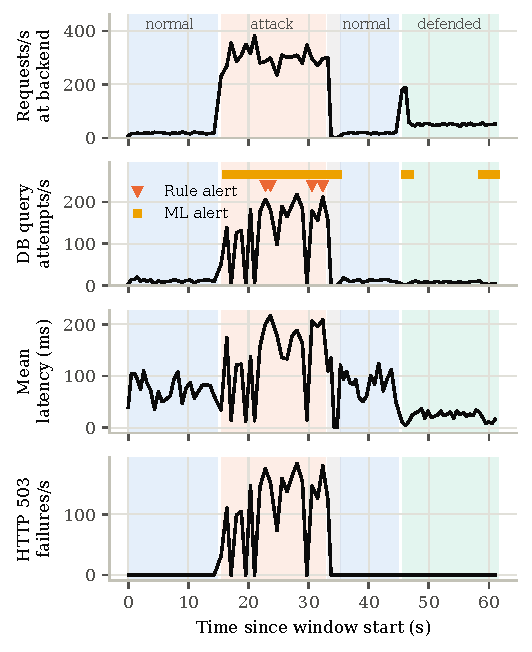
\includegraphics[width=\columnwidth]{figures/fig_timeline.pdf}
\caption{Representative 60~s window: normal, undefended attack, normal, defended
attack. Markers show rule and ML alerts.}
\label{fig:timeline}
\end{figure}

\begin{figure}[t]
\centering
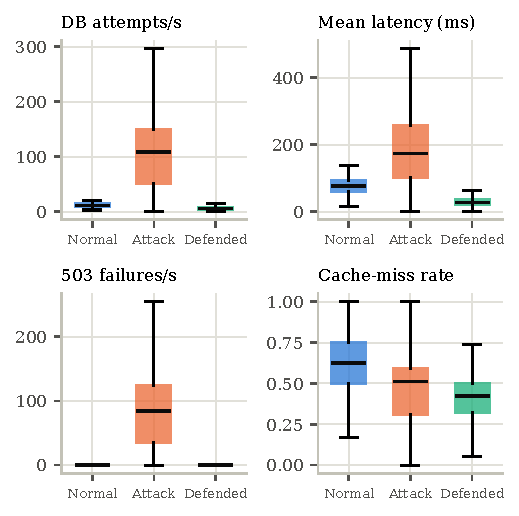
\includegraphics[width=\columnwidth]{figures/fig_boxplots.pdf}
\caption{Per-interval distributions under the three conditions (outliers omitted).}
\label{fig:boxplots}
\end{figure}

\textbf{Undefended attack.} Well-formed requests for existing products raised database
attempts from 11 to a median of 108/s (9.8$\times$; peak 317, 28.8$\times$), more than
doubled median latency to 174~ms (p95 450~ms, max 1.16~s), and produced 503s in 79.7\%
of intervals (median 84/s, max 274/s). In total, 79\% of 77{,}408 database attempts were
rejected. This answers RQ1.

\textbf{Defended attack.} The same attack left the database at 6~q/s, consistent with
Eq.~\eqref{eq:defended}. That is below the baseline, because the edge limiter also
throttles the synthetic normal traffic that shares the load generator's address. The
backend rate was pinned at 50~req/s, median latency fell to 27~ms (p95 84~ms), and only
419 failures occurred in 35{,}272 intervals, at mode transitions. Median database load
fell \textbf{18.0$\times$} (95\% CI 16.8--19.2) and median latency \textbf{6.4$\times$}
(CI 6.1--6.8). We report ratios of medians because peak-to-typical ratios (e.g.\
$317/6\approx53\times$) overstate the effect. Defended latency was even below baseline
(IQRs 20--37 vs.\ 61--94~ms), since lock losers are served from Redis, at the cost of up
to 60~s of staleness. During the 4.5~h soak, median load was 6~q/s (p99 15), latency
27~ms (p99 140~ms), and only one interval had failures.

\subsection{Overload Mechanics: Goodput Collapse (RQ2)}
\label{sec:mechanics}
Fig.~\ref{fig:saturation} shows that undefended intervals lie on a line of slope
${\approx}1$. Beyond ${\approx}20$--$25$ attempts/s, every extra attempt fails.
Completed database queries stay near a median of 23/s, about a fifth of the nominal
$\mu_{\max}\approx109$~q/s. Three mechanisms explain this collapse
\cite{jacobson1988,mogul1997}: (i)~the fail-fast pool rejects all but 12 of a 250-request
burst instantly; (ii)~failed regenerations never fill the cache, so the burst
re-stampedes the same key; and (iii)~200 threads share one Python interpreter, so
failing requests steal CPU from those holding connections. The database is thus
overwhelmed long before its nominal capacity.

\begin{figure}[t]
\centering
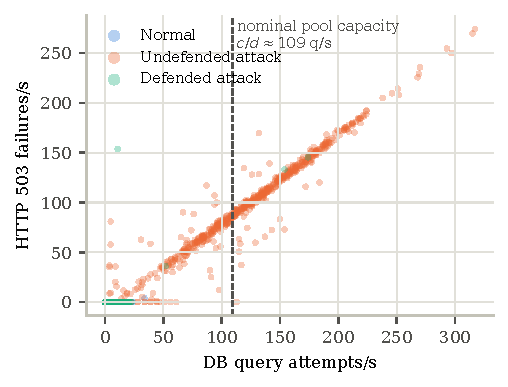
\includegraphics[width=\columnwidth]{figures/fig_db_saturation.pdf}
\caption{503 failures vs.\ database attempts per interval. Under attack, failures grow
one-for-one with attempts far below nominal pool capacity (dashed).}
\label{fig:saturation}
\end{figure}

\subsection{Mitigation, Ablation, and Recovery (RQ4)}
\label{sec:ablation}
Locking raises the coalescing ratio from 1.00 to 4.70 (592{,}029 misses, 125{,}957
attempts): about five concurrent misses share each regeneration, and none waits. The
edge limiter cuts the backend rate from 250 to exactly 50~req/s.
Table~\ref{tab:ablation} shows the ablation. Locking alone protected the database but,
with losers waiting, latency reached ${\approx}2.5$~s; SWR removed that queue. Yet the
storefront stayed slow and variable, because the flood still consumed proxy connections
and application threads. Only edge limiting made it consistently fast.
\emph{Database protection and request-path protection are distinct problems.}

\begin{table}[t]
\centering
\caption{Mitigation ablation under attack (storefront = per-item load time).}
\label{tab:ablation}
\footnotesize
\setlength{\tabcolsep}{3pt}
\begin{tabularx}{\columnwidth}{@{}L{2.3cm}L{1.5cm}YL{1.3cm}@{}}
\toprule
Configuration & DB load & Storefront & Availability \\
\midrule
No defense & 108 att./s & Fails or 300--500 ms & Denied \\
Lock only (wait) & 1--4 q/s & Up to $\approx$2.5 s & Degraded \\
+ SWR & Protected & 80--140 ms, variable & Degraded \\
+ Edge limit & 6 q/s & 20--140 ms & Preserved \\
\bottomrule
\end{tabularx}
\end{table}

Fig.~\ref{fig:dev} confirms this across 14 sessions. Median defended latency fell from
105--107~ms (early) to 65--91~ms, then to 26--32~ms once SWR and real client-address
forwarding were in place. The defended backend rate stayed at 170--350~req/s until the
final session, when the edge limiter pinned it at 50. Undefended attacks stayed severe
throughout (96--351~ms).

\begin{figure}[t]
\centering
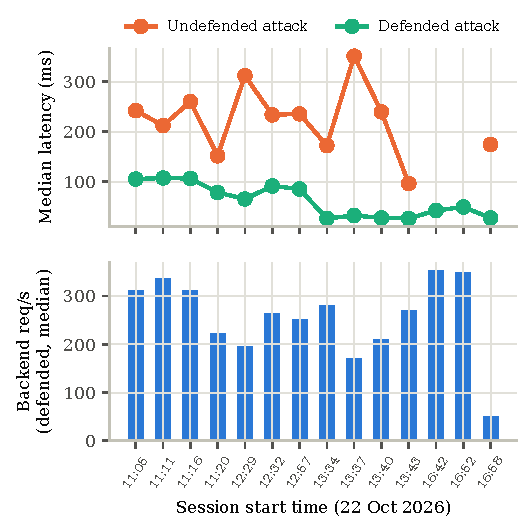
\includegraphics[width=\columnwidth]{figures/fig_dev_evolution.pdf}
\caption{Longitudinal view of 14 sessions: median latency under attack (top) and backend
request rate under defended attack (bottom).}
\label{fig:dev}
\end{figure}

\textbf{Recovery.} Enabling defenses mid-attack restored health after a median of
1.35~s (max 2.77~s; 7 transitions). Stopping an attack restored health in a median of
1.08~s (max 2.51~s; 26 of 31 transitions observable). This meets G4.

\subsection{Detection (RQ3)}
\label{sec:det-results}
\textbf{Episodes.} Over the final session's 12 attack episodes (Fig.~\ref{fig:detlat}),
the rule detected 11 with median latency 3.2~s (IQR 2.4--5.6, max 18.1). The
IsolationForest detected 10, with median 0.85~s (IQR 0--1.0, max 1.3). One ML miss came
before any normal traffic had trained the model; the other came just after training on
a very short window. Their misses do not overlap, so the union detected \textbf{all 12}
(median 0.95~s).

\begin{figure}[t]
\centering
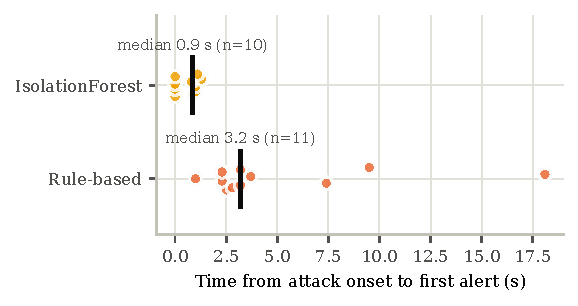
\includegraphics[width=\columnwidth]{figures/fig_detect_latency.pdf}
\caption{Detection latency per attack episode; bars mark medians.}
\label{fig:detlat}
\end{figure}

\textbf{Intervals.} Table~\ref{tab:det} shows that the rule is perfectly precise but
fires on only 27\% of attack intervals, because the bursty attack aligns its three
conditions only intermittently. The forest reaches recall 0.91 (0.94 once trained) with
one false positive in 332. The OR combination gives F1 0.96.

\begin{table}[t]
\centering
\caption{Interval-level detection (733 attack / 332 normal) and alert rate in other
modes, final session.}
\label{tab:det}
\footnotesize
\setlength{\tabcolsep}{2.5pt}
\begin{tabular}{@{}lcccc|cc@{}}
\toprule
Detector & Prec. & Rec. & F1 & FPR & Idle & Defended \\
\midrule
Rule & 1.000 & 0.274 & 0.430 & 0.000 & 0.0001 & 0.000 \\
IsolationForest & 0.999 & 0.914 & 0.954 & 0.003 & 0.993 & 0.128 \\
Rule OR IForest & 0.999 & 0.925 & 0.960 & 0.003 & -- & -- \\
\bottomrule
\end{tabular}
\end{table}

\textbf{Idle and defended traffic.} The forest fired in 99.3\% of idle intervals and
12.8\% of defended ones; the rule fired in neither. The idle result is the closed-world
problem \cite{sommer2010}: a model trained on traffic treats \emph{no} traffic as
abnormal. The detectors answer different questions. The rule asks \emph{``is the
database being harmed?''}; the forest asks \emph{``does traffic look unfamiliar?''}.

\textbf{Harm vs.\ volume.} Table~\ref{tab:single} tests each signal alone. A volume
threshold looks excellent on attack-vs-normal (F1 0.98), because attack volume is
${\approx}14\times$ normal here. But it fires on 97.1\% of absorbed-burst intervals,
where the rule and the database-load condition never fire. \emph{Volume detects
traffic; the rule detects harm.} The table also exposes a design flaw: the normal miss
ratio is already high (Section~\ref{sec:model}), so ``miss ratio $>0.5$'' has a 67\%
FPR alone, and inside the conjunction it only removes true positives. Database load
alone (F1 0.85) and the presence of 503s (F1 0.89) are each stronger than the deployed
three-way rule.

\begin{table}[t]
\centering
\caption{Single-signal detectors (attack vs.\ normal) and firing rate on 2{,}080
absorbed-burst (harmless, high-volume) intervals.}
\label{tab:single}
\footnotesize
\setlength{\tabcolsep}{3pt}
\begin{tabular}{@{}lcccc@{}}
\toprule
Detector & Rec. & F1 & FPR & Absorbed \\
\midrule
Volume: rps $>100$ & 0.966 & 0.983 & 0.000 & 97.1\% \\
DB load $>5\times$ base & 0.739 & 0.850 & 0.000 & 0.0\% \\
Latency $>200$ ms & 0.404 & 0.575 & 0.000 & 0.8\% \\
Miss ratio $>0.5$ & 0.531 & 0.578 & 0.672 & 8.3\% \\
Any 503 & 0.797 & 0.886 & 0.003 & 0.0\% \\
Rule (all three) & 0.274 & 0.430 & 0.000 & 0.0\% \\
\bottomrule
\end{tabular}
\end{table}

\textbf{Thresholds.} Fig.~\ref{fig:rulegrid} shows that recall is governed by $\tau_L$.
At 100~ms recall rises to 0.51, while the FPR stays $\le$0.9\% across the grid. The
best F1 over the full grid is 0.82 (precision 0.99, recall 0.70), at $K=2$,
$\tau_L=100$~ms, $\tau_m=0.3$. The deployed thresholds are conservative.

\begin{figure*}[t]
\centering
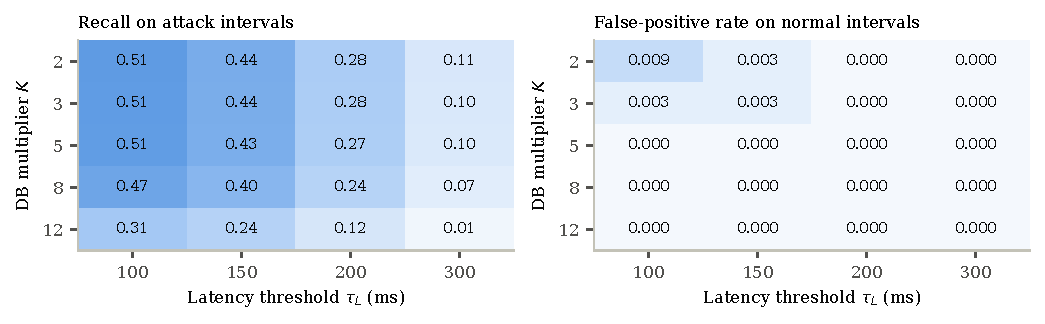
\includegraphics[width=0.85\textwidth]{figures/fig_rule_grid.pdf}
\caption{Rule threshold sensitivity ($\tau_m=0.5$): recall on attack intervals (left) and
false-positive rate on normal intervals (right).}
\label{fig:rulegrid}
\end{figure*}

\textbf{Offline IsolationForest.} The replayed forest reaches ROC AUC 0.999 (0.994--1.000
over 10 seeds; Fig.~\ref{fig:roc}), so its ranking is excellent and only the operating
point varies. Contamination 0.01 gives recall 0.989 at a held-out FPR of 1.8\%; 0.03
gives recall 1.0 but an FPR of 11.5\%. Request rate alone ranks almost as well (AUC
0.995), while the miss ratio is inversely related to attack (AUC 0.25). The forest's
fragility is training size. Recall was 0.16 with the deployed 10-sample minimum, 0.90
with 20, 0.22 with 100, and 0.99 with 166. The learned threshold depends on which normal
intervals the window happens to contain, so a longer minimum window and a
validation-set threshold are needed.

\begin{figure}[t]
\centering
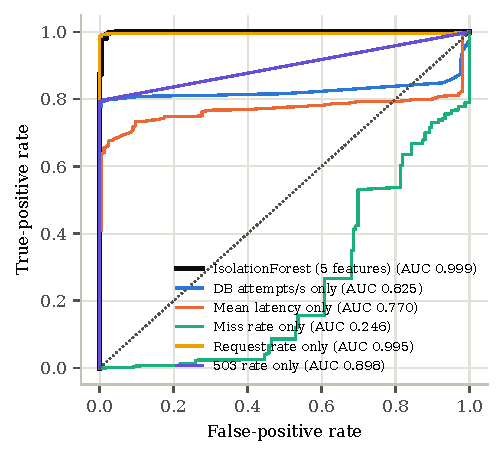
\includegraphics[width=\columnwidth]{figures/fig_roc.pdf}
\caption{ROC on held-out intervals: IsolationForest vs.\ each feature alone.}
\label{fig:roc}
\end{figure}

\subsection{End-to-End Validation}
All 16 automated tests passed. They cover container health, routing, caching (137 vs.\
9~ms), 404 handling, a calm baseline (peak 17~q/s, 0 alerts), overload under attack
(227~q/s, 145 failures per interval), both detectors firing, protection (11~q/s, 0
failures), recovery (${\approx}2$~s), live-feed rate, controls, and 20/20 storefront
requests served during a defended attack.

%% =====================================================================
\section{Discussion}
\label{sec:discussion}
%% =====================================================================

\subsection{Why the Defense Must Be Layered}
Locking is the only control that removes the root cause, restoring $N{:}1$ to $1{:}1$.
SWR makes it fast. Application limiting acts too late, after the proxy and application
have paid for the request. Edge limiting protects the proxy but does not remove
amplification of what it admits. The right order follows the request: edge limit,
then coalesce, then serve stale. This mirrors early load shedding
\cite{welsh2001,beyer2016} and prevention--detection--response \cite{zargar2013}.
Table~\ref{tab:mitig} compares the alternatives. Jitter, longer TTLs, and early
recomputation reduce the \emph{chance} of a synchronized miss, but a timing attacker
defeats them; a secure design must also bound the \emph{cost} of a stampede.

\begin{table}[t]
\centering
\caption{Stampede mitigations. RC = removes root cause; Proxy = protects request path;
Adv.\ = effective against timed bursts.}
\label{tab:mitig}
\footnotesize
\setlength{\tabcolsep}{3pt}
\begin{tabularx}{\columnwidth}{@{}L{2.5cm}cccY@{}}
\toprule
Technique & RC & Proxy & Adv. & Caveat \\
\midrule
Longer TTL / jitter & \no & \no & \no & Fewer, not smaller stampedes \\
XFetch \cite{vattani2015} & \prt & \no & \prt & Needs cost estimate \\
Lock / lease \cite{nishtala2013} & \yes & \no & \yes & Losers must be served \\
SWR \cite{rfc5861} & \prt & \no & \yes & Needs stale copy \\
App rate limit & \no & \no & \prt & Acts after the proxy \\
Edge rate limit \cite{nginxlimitreq} & \no & \yes & \yes & Per address \\
Auto-scaling & \no & \prt & \no & Slow; Yo-Yo \cite{sides2016} \\
\textbf{All combined (ours)} & \yes & \yes & \yes & Bounded staleness \\
\bottomrule
\end{tabularx}
\end{table}

\subsection{Harm Detection vs.\ Novelty Detection}
The rule detects harm: it stays silent on absorbed bursts, defended attacks, and
idleness. The forest detects novelty: it is fast and dense, but it also flags idleness.
Both are useful. A deployment should page operators on the rule and send the forest's
alerts to a security dashboard, where a defended attack is still worth seeing. The
forest also needs a ``no traffic'' state. The miss-ratio result carries a further
lesson: a signal that sounds right (``misses spike during a stampede'') can be wrong
under realistic TTLs. Features should be validated against a model of normal behavior,
and signals that measure the protected resource directly are preferable.

\subsection{Engineering Lessons}
\label{sec:lessons}
Several key results first surfaced as bugs (Table~\ref{tab:bugs}).

\begin{table}[t]
\centering
\caption{Defects found during development and their lessons.}
\label{tab:bugs}
\footnotesize
\setlength{\tabcolsep}{3pt}
\begin{tabularx}{\columnwidth}{@{}L{2.6cm}Y@{}}
\toprule
Symptom $\rightarrow$ cause & Fix / lesson \\
\midrule
Attacker throttled real users $\rightarrow$ limiter saw only the proxy's address & Overwrite \texttt{X-Forwarded-For}; per-client limits need trusted identity \\
Defended latency ${\approx}$2.5 s $\rightarrow$ lock losers queued & Serve stale + pre-warm; coalescing must not become queueing \\
Shop slow with DB protected $\rightarrow$ flood congested proxy & Edge \texttt{limit\_req}; protect the request path \\
False alarm at start $\rightarrow$ cold cache mimics attack & 3 s warm-up suppression; keep it out of ML training \\
ML blips $\rightarrow$ single noisy samples & Two-interval debounce; contamination 0.03$\rightarrow$0.01 \\
Inconsistent metrics $\rightarrow$ several Gunicorn workers & One worker, 200 threads \\
Shop stuck after attack $\rightarrow$ fetches without timeout & 4 s timeout, non-overlapping refresh \\
\bottomrule
\end{tabularx}
\end{table}

\textbf{Deployment guidance.} (1)~Coalesce hot-key regeneration, with token-checked
locks \cite{kleppmann2016}. (2)~Keep and pre-warm stale copies. (3)~Rate-limit at the
edge and return 429 for intentional shedding. (4)~Forward trusted client identity.
(5)~Choose pool behavior deliberately: fail-fast sheds load but hurts goodput.
(6)~Monitor the protected resource---database attempts, pool exhaustion, failures---not
proxies such as miss ratio. (7)~Run a harm detector and a novelty detector, and train
the latter on a clean, sufficiently long window. (8)~Treat TTLs as public.

\textbf{Ethics.} Attack traffic targets only the stack's own proxy on a private network,
and all data are synthetic. The control API is unauthenticated and Grafana uses default
credentials, which is acceptable only locally. Any reachable deployment must be
firewalled to known addresses and use changed passwords.

\subsection{Threats to Validity and Limitations}
\label{sec:validity}
\emph{Construct:} ``DB queries'' are attempts, including rejected ones; failures are
logged per interval; hits and misses overlap under defense; latency is measured inside
the application, so edge rejections (503 by default) are invisible; p95 is quantized to
histogram buckets; per-container CPU and memory were specified but not collected; and
the active defense set is not logged per interval, so the ablation is partly
observational. \emph{Internal:} attacker, victim, and monitor share one host, and mode
labels can lag traffic by one interval. \emph{External:} this is a single-host Docker
Desktop setup with synthetic, uniform popularity and \texttt{pg\_sleep} cost. All
synthetic traffic comes from one address, so the edge limiter also throttles normal
traffic, and per-address limiting is easier than against a distributed attacker.
Legitimate-user availability under defense is therefore evidenced by the storefront and
test~16, which come from a different address. \emph{Conclusion:} intervals are
autocorrelated, so interval-level CIs are optimistic; the episode-level and
cross-session results are the conservative evidence. The forest needs a clean baseline,
and all thresholds need site-specific calibration.

\subsection{Complex Engineering Problem Attributes}
Following \cite{ieagapc2021}, the project spans: depth of knowledge (caching, queueing,
rate limiting, anomaly detection); conflicting requirements (database protection vs.\
latency vs.\ freshness vs.\ false alarms); depth of analysis (analytical model,
statistics, ROC, ablation); unfamiliar issues (a performance hazard reframed as an
unpatchable attack); applicable codes (RFC~6585/5861, OWASP, ATT\&CK, NIST); multiple
stakeholders (users, operators, analysts); and interdependence (nine services, with
defenses effective only in combination).

%% =====================================================================
\section{Conclusion}
\label{sec:conclusion}
%% =====================================================================
CacheCollapse shows that a cache stampede is a practical indirect denial-of-service
attack, and that it can be both detected and defeated with standard components.
\textbf{RQ1:} rotating 250-request bursts raised median database attempts ${\approx}10\times$
and caused 503s in 80\% of intervals. \textbf{RQ2:} a simple model predicts baseline load
within 9\%; under attack, a fail-fast pool and unfilled regenerations collapse goodput to
${\approx}23$~q/s, a fifth of nominal capacity. \textbf{RQ3:} the rule (precision 1.0,
median 3.2~s) and the IsolationForest (recall 0.91, median 0.85~s) together caught 12 of
12 attacks with one false alarm. The rule detects harm and ignores absorbed bursts that a
volume threshold flags 97\% of the time. \textbf{RQ4:} locking with SWR plus app and edge
limiting cut database load 18$\times$ and latency 6.4$\times$, held for 4.5~h, and
recovered in 1.35~s. Both database-level and edge-level controls are required.

Future work: Zipf-distributed trace replay; distributed attackers with aggregate and
adaptive admission control \cite{welsh2003,ranjan2009}; multi-node Kubernetes with
auto-scaling \cite{sides2016,bremlerbarr2017}; early recomputation \cite{vattani2015}; a
rule based on pool exhaustion instead of miss ratio, with automatically calibrated
thresholds; and per-container resource and proxy-side latency metrics.

\section*{CRediT Authorship Contribution Statement}
\textbf{Manal Aamir:} Conceptualization, Methodology, Writing -- Review and Editing.
\textbf{Tayyaba Arshad:} Investigation, Validation, Data Curation.
\textbf{Noor Afza:} Software (load generation and monitoring), Visualization.
\textbf{Batool Fatima:} Software (detection and mitigation), Validation.
\textbf{Aun Zaidi:} Conceptualization, Methodology, Software (system integration),
Writing -- Original Draft.

%% NOTE TO AUTHORS: edit or delete this declaration to match your actual use.
\section*{Declaration of AI-Assisted Tools}
AI-assisted tools were used to help analyze the experiment logs, generate figures, and
draft and edit parts of the text. The authors reviewed and edited all content and take
full responsibility for it.

\bibliographystyle{IEEEtran}
\bibliography{references}

\end{document}
